\documentclass[12pt]{standalone}
\usepackage[utf8]{inputenc}
\usepackage[T1]{fontenc}
\usepackage{times}
\usepackage{amsmath,amssymb}
\usepackage[dvipsnames,svgnames]{xcolor}
\usepackage{tikz}
\usetikzlibrary{decorations.pathreplacing, calc, positioning, shapes.geometric, shapes.symbols, arrows.meta, backgrounds, fit, shapes.misc}
\definecolor{RED}{rgb}{1,0,0}
\definecolor{dmrsfill}{HTML}{CDE2FB}
\definecolor{winblue}{HTML}{0D366B}
\definecolor{inksec}{HTML}{52514E}
\begin{document}
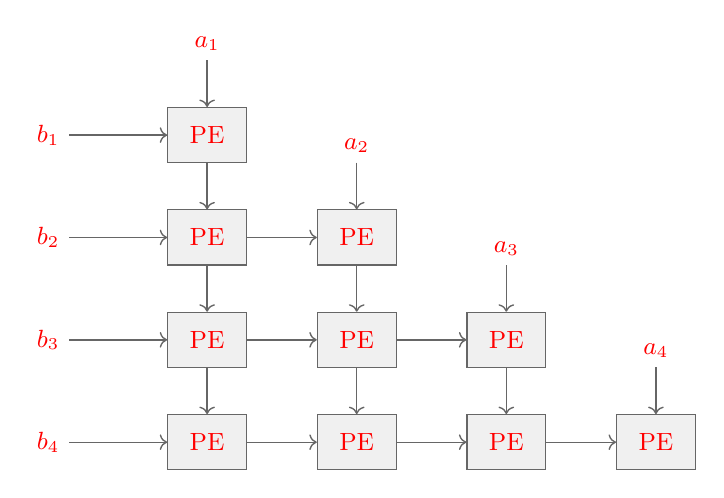
\begin{tikzpicture}[font=\small,
  every node/.append style={text=red},
  pe/.style={draw=black!60, fill=black!6, minimum width=1.0cm, minimum height=0.7cm, inner sep=0pt, line width=0.4pt},
  seta/.style={black!60, ->, line width=0.5pt}]
\def\dx{1.9}\def\dy{1.3}
\foreach \i in {1,...,4} {
  \foreach \j in {1,...,\i} {
    \node[pe] (p\i\j) at (\j*\dx, -\i*\dy) {PE};
  }
}
% entradas pela esquerda (b) e por cima (a)
\foreach \i in {1,...,4} {
  \draw[seta] (0.15, -\i*\dy) node[left] {$b_{\i}$} -- (p\i1.west);
  \draw[seta] (\i*\dx, -\i*\dy+0.95) node[above] {$a_{\i}$} -- (p\i\i.north);
}
% passagem para a direita e para baixo
\foreach \i in {2,...,4} {
  \pgfmathtruncatemacro{\im}{\i-1}
  \foreach \j in {1,...,\im} {
    \pgfmathtruncatemacro{\jp}{\j+1}
    \draw[seta] (p\i\j.east) -- (p\i\jp.west);
    \draw[seta] (p\im\j.south) -- (p\i\j.north);
  }
}
\end{tikzpicture}
\end{document}
